\documentclass[10pt] {article}
\usepackage{fullpage}
\usepackage{amssymb}
\usepackage{graphicx}
\usepackage{float}
\usepackage{amsthm}
\usepackage{qtree}
\usepackage{hyperref}
\usepackage{amsmath}
\renewcommand\qedsymbol{$\blacksquare$}

\title{Homework 4 }
\author{Ricky Hempel}
\begin{document}
\maketitle
\begin{center}
Chapter 1: 1.19
Chapter 2: 2.1, 2.4, 2.6acd, 2.8, 2.13a, 2.14
\end{center}
\begin{enumerate}
\item[1.19]a.$(0 \cup 1)^{*}000(0 \cup 1)^*$
\begin{figure}[H]
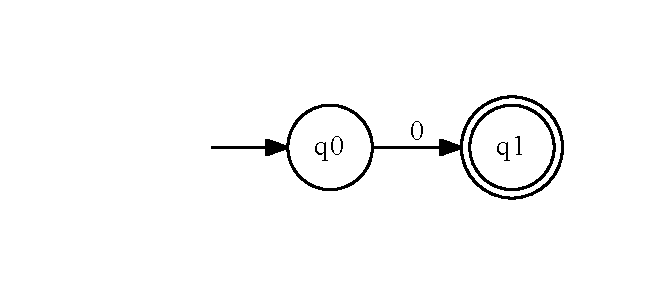
\includegraphics[width=0.5\textwidth]{aa19.pdf}
\caption{The NFA for 0.}
\label{1}
\end{figure}
\begin{figure}[H]
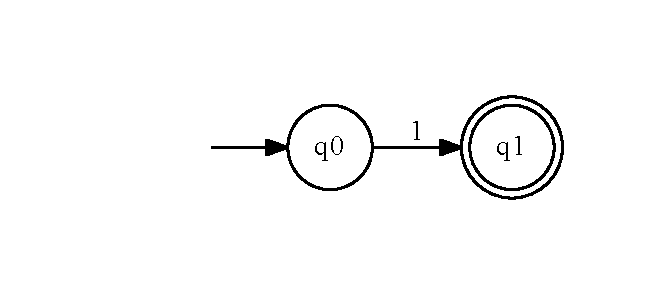
\includegraphics[width=0.5\textwidth]{ab19.pdf}
\caption{The NFA for 1.}
\label{2}
\end{figure}
\begin{figure}[H]
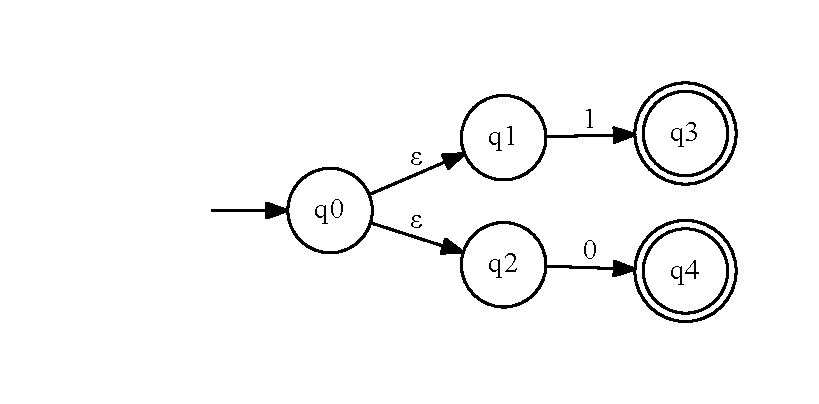
\includegraphics[width=0.5\textwidth]{ac19.pdf}
\caption{The NFA for 0 $\cup$ 1.}
\label{3}
\end{figure}
\begin{figure}[H]
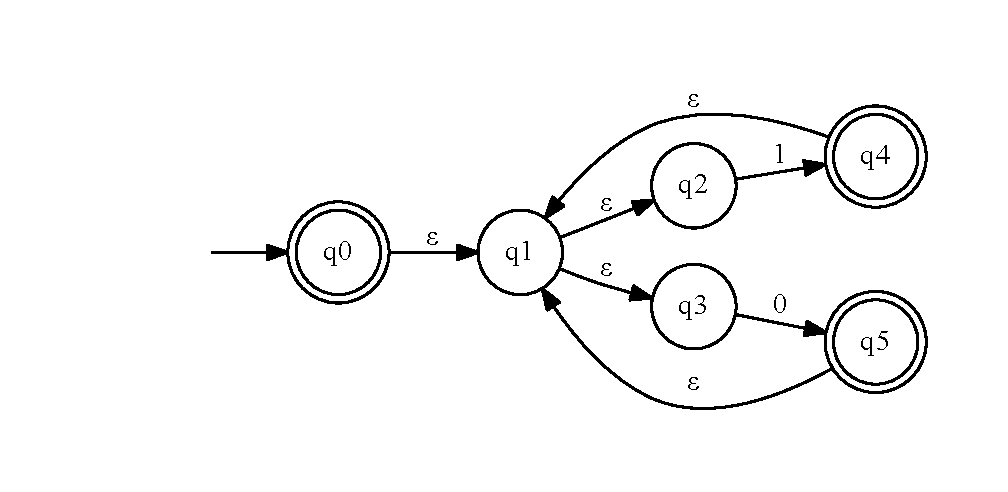
\includegraphics[width=0.7\textwidth]{ad19.pdf}
\caption{The NFA for (0 $\cup$ 1)*.}
\label{4}
\end{figure}
\begin{figure}[H]
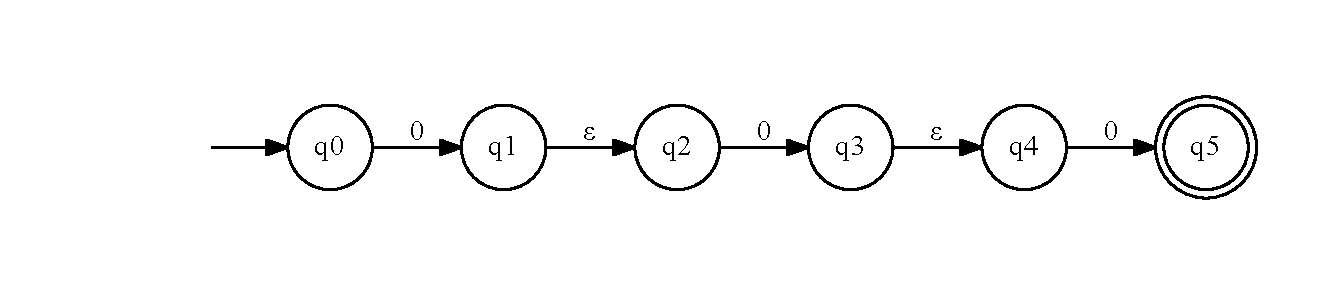
\includegraphics[width=0.8\textwidth]{ae19.pdf}
\caption{The NFA for 000.}
\label{5}
\end{figure}
\begin{figure}[H]
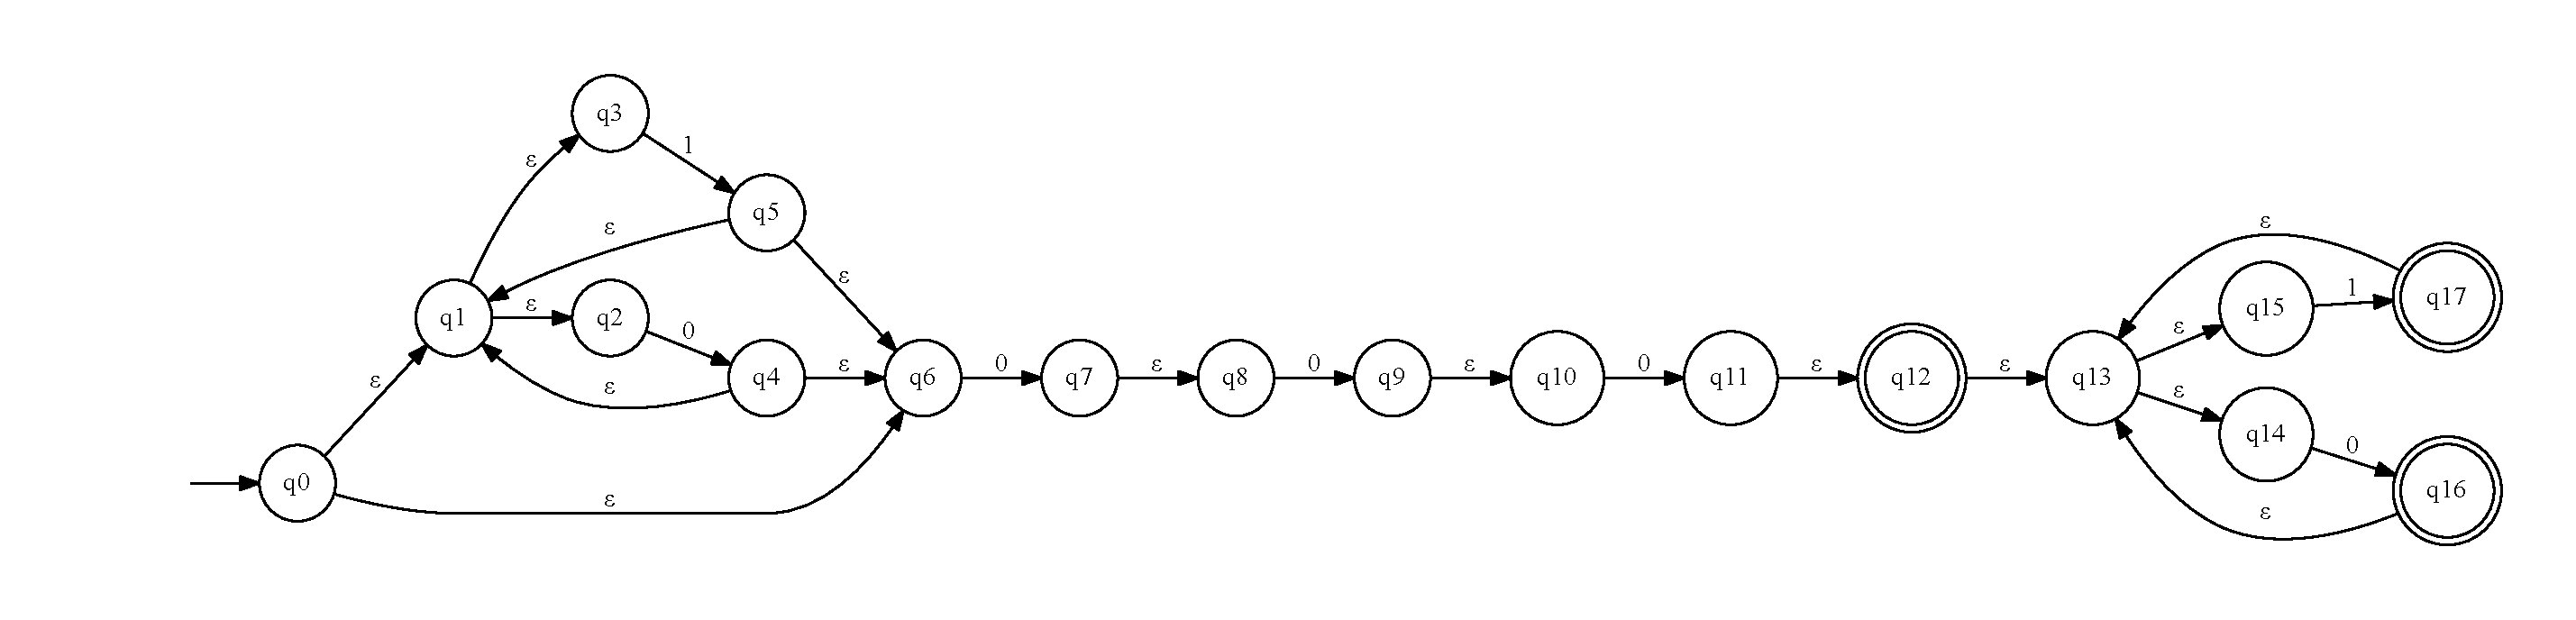
\includegraphics[width=0.9\textwidth]{af19.pdf}
\caption{The NFA for $(0 \cup 1)^*000(0 \cup 1)^*$.}
\label{6}
\end{figure}
b.$(((00)^*(11))\cup 01)^*$
\begin{figure}[H]
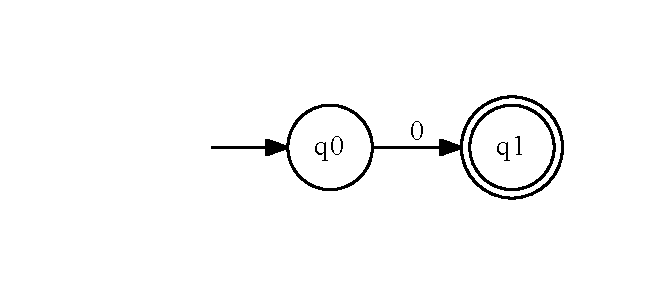
\includegraphics[width=0.5\textwidth]{aa19.pdf}
\caption{The NFA for 0.}
\label{7}
\end{figure}
\begin{figure}[H]
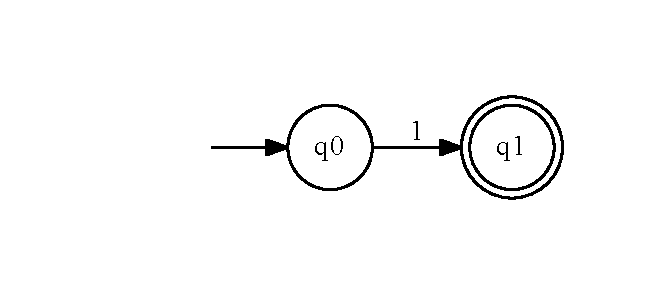
\includegraphics[width=0.5\textwidth]{ab19.pdf}
\caption{The NFA for 1.}
\label{8}
\end{figure}
\begin{figure}[H]
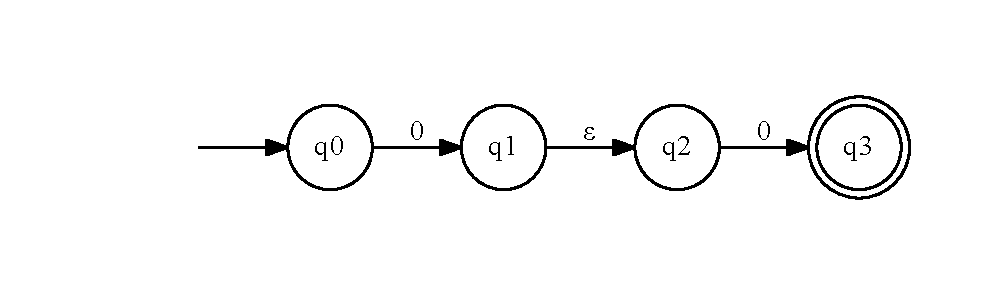
\includegraphics[width=0.8\textwidth]{ba19.pdf}
\caption{The NFA for 00.}
\label{9}
\end{figure}
\begin{figure}[H]
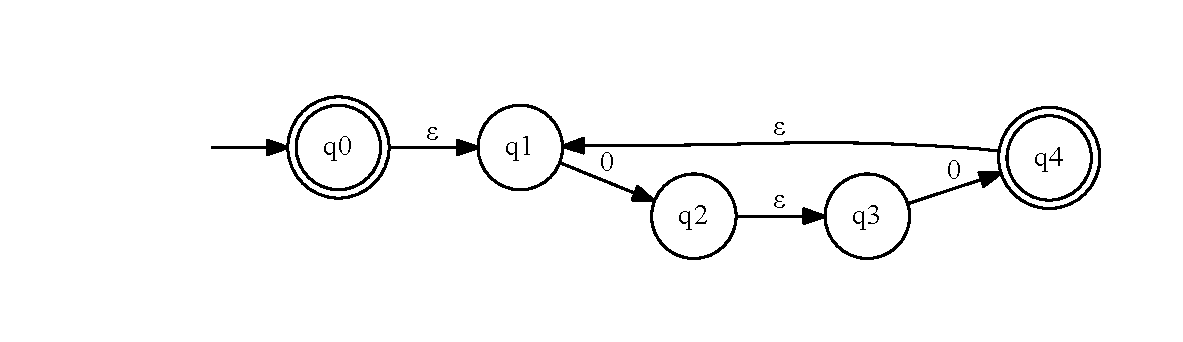
\includegraphics[width=0.8\textwidth]{bc19.pdf}
\caption{The NFA for (00)*.}
\label{10}
\end{figure}
\begin{figure}[H]
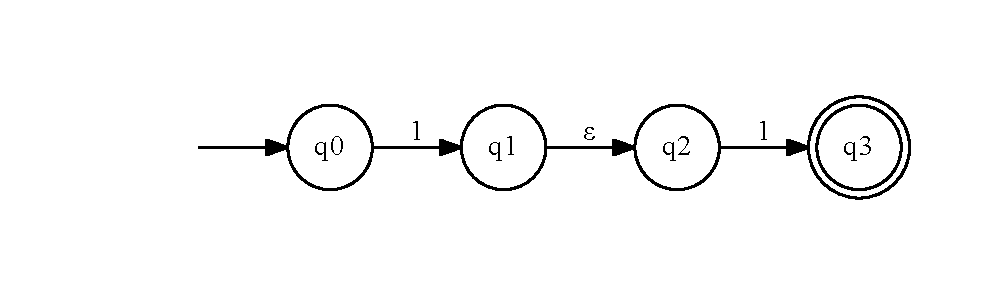
\includegraphics[width=0.8\textwidth]{bd19.pdf}
\caption{The NFA for 11.}
\label{11}
\end{figure}
\begin{figure}[H]
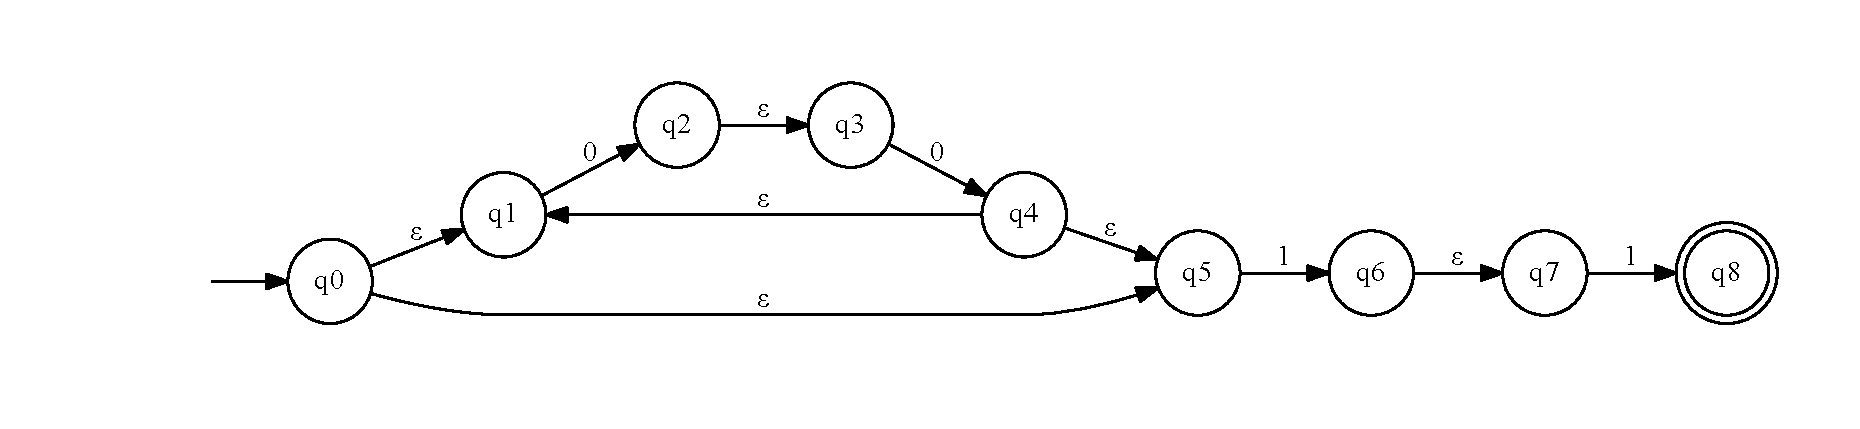
\includegraphics[width=0.9\textwidth]{be19.pdf}
\caption{The NFA for (00)*11.}
\label{12}
\end{figure}
\begin{figure}[H]
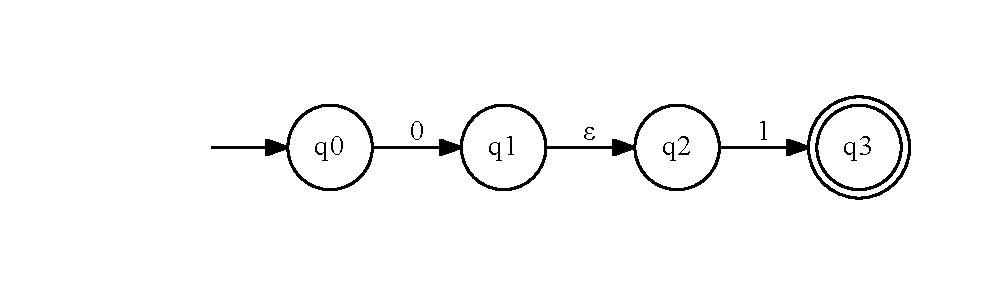
\includegraphics[width=0.9\textwidth]{bf19.pdf}
\caption{The NFA for 01.}
\label{13}
\end{figure}
\begin{figure}[H]
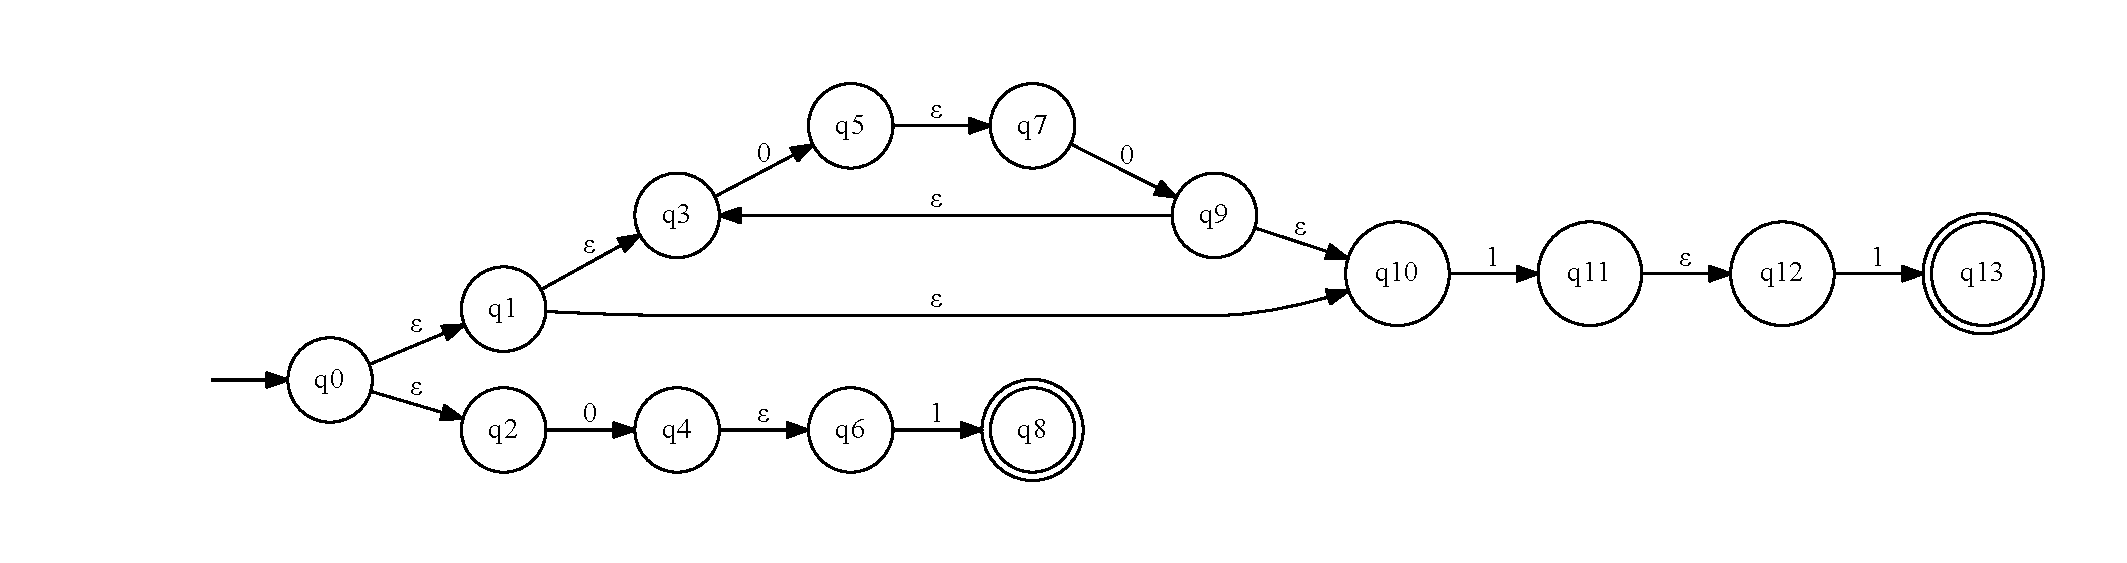
\includegraphics[width=0.9\textwidth]{bg19.pdf}
\caption{The NFA for (((00)*(11))$\cup$(01)).}
\label{14}
\end{figure}
\begin{figure}[H]
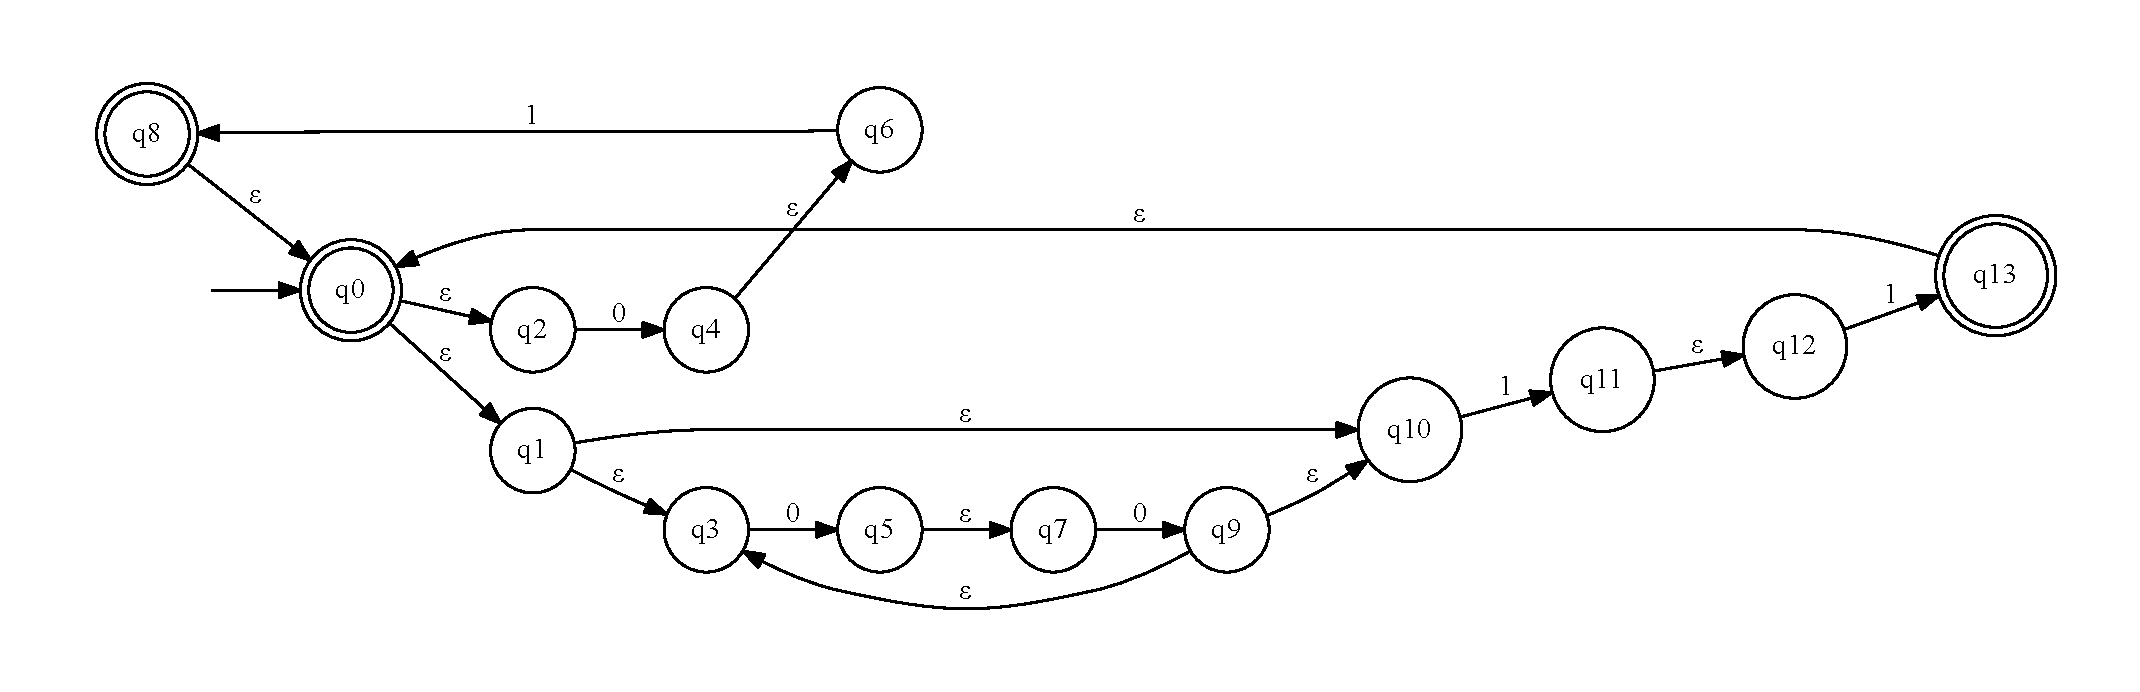
\includegraphics[width=0.9\textwidth]{bh19.pdf}
\caption{The NFA for (((00)*(11))$\cup$(01))*.}
\label{15}
\end{figure}
c.$\emptyset^*$
\begin{figure}[H]
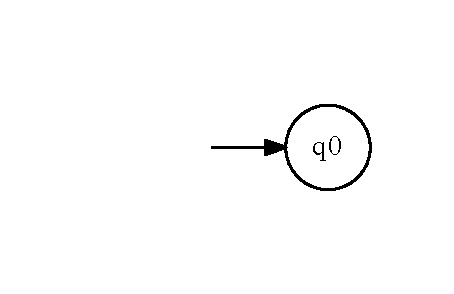
\includegraphics[width=0.5\textwidth]{c.pdf}
\caption{The NFA for $\emptyset$.}
\label{21}
\end{figure}
\begin{figure}[H]
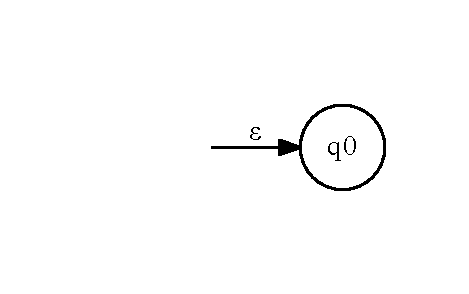
\includegraphics[width=0.5\textwidth]{ca.pdf}
\caption{The NFA for $\emptyset^*$.}
\label{16}
\end{figure}
\item[2.1]a.
The derivation for a  is $E \Rightarrow T \Rightarrow F \Rightarrow a$
and the parse tree is below.
\begin{align*}
\Tree[.E [.T [.F \textit{a} ]]
            ]
            \end{align*}
b.The derivation for a+a is $E \Rightarrow E+T \Rightarrow T+T \Rightarrow T+F \Rightarrow F + a \Rightarrow a+a  $ and the parse tree is below.
\begin{align*}
\Tree[ [  [ [ a ].F ].T ].E + [ [ a ].F ].T ].E 
\end{align*}
c.The derivation for a+a is $E \Rightarrow E+T \Rightarrow E+T+T \Rightarrow T+T+T \Rightarrow F + T+T \Rightarrow F+F+T \Rightarrow F+F+F \Rightarrow a+F+F \Rightarrow a+a+F \Rightarrow a+a+a  $ and the parse tree is below.
\begin{align*}
\Tree[ [  [ [ [ a ].F ].T ].E + [ [ a ].F ].T ].E + [ [ a ].F ].T ].E
\end{align*}
d..The derivation for ((a)) is $E \Rightarrow T \Rightarrow F \Rightarrow (E) \Rightarrow (T) \Rightarrow (F) \Rightarrow ((E)) \Rightarrow ((T)) \Rightarrow ((F)) \Rightarrow ((a))  $ and the parse tree is below.

\Tree[ [ [ ( [ [ [ ( [ [ [ a ].F ].T ].E ) ].F ].T ].E ) ].F ].T  ].E
\item[2.4]
a.$S \rightarrow Q1Q1Q1Q$\\
$Q\rightarrow 0Q \mid 1Q \mid \varepsilon$\\
b.$S \rightarrow 0Q0 \mid 1Q1 \mid 0 \mid 1$\\
$Q \rightarrow 0Q \mid 1Q \mid \varepsilon$\\
c.$S \rightarrow 0 \mid 1 \mid 00S \mid 01S \mid 10S \mid 11S $\\
d.$S \rightarrow 0 \mid 0S0 \mid 0S1 \mid 1S0 \mid 1S1$\\
e.$S \rightarrow 0 \mid 1 \mid 0S0 \mid 1S1 \mid \varepsilon$\\
f.$S \rightarrow S$
\item[2.6]
a.$S \rightarrow YaY$\\
$Y \rightarrow YY \mid aYb \mid bYa \mid a \mid \varepsilon$\\
c.$S \rightarrow QR$\\
$Q \rightarrow 0Q0 \mid 1Q1 \mid \#R$ \\
$R \rightarrow 0R \mid 1R \mid \varepsilon$\\
d.$S \rightarrow Q \mid Y \# Q \# Y \mid Y \# Q\mid Q \#Y$\\
$Q \rightarrow aQa\mid bQb \mid \# \mid \#Y \#$\\
$Y \rightarrow aY \mid bY \mid \#Y \mid \varepsilon$
\item[2.8]In the first derivation the sentence means that the girl used the flower to touch the boy. In the second derivation, the boy is holding the flower when the boy touches her.
\begin{align*}
\Tree[ [ [ [ the ].Article [ girl ].Noun ].Complex-Noun ].Noun-Phrase [  [ touches [ [ [ the ].Article [ boy ].Noun   ].Complex-Noun [ [ with ].Preposition [ [ the ].Article [ flower ].Noun ].Complex-Noun ].Preposition-Phrase ].Noun-Phrase ].Complex-Verb ].Verb-Phrase ].Sentence
\end{align*}
\begin{align*}
\Tree[ [ [ [ the ].Article [ girl ].Noun ].Complex-Noun ].Noun-Phrase [ [ touches [ [ [ the ].Article [ boy ].Noun ].Complex-Noun ].Noun-Phrase ].Complex-Verb [ [ with ].Prepostion [ [ the ].Article [ flower ].Noun ].Complex-Noun ].Preposition-Phrase ].Verb-Phrase  ].Sentence
\end{align*}
\item[2.13]
a.The language generated by $L=L(G)$ is the set of strings such that either they are composed by the concatenation of 3 or more arbitrary-length strings of zeros (delimited by the $\#$ symbol) or strings of the form $0^k\#0^{2k}$ for $k \geq 0$.
\item[2.14] First add a new start variable $S_0$ and the rule $S_0 \rightarrow A$.
Now the grammar is.\\
$S_0 \rightarrow A$\\
$A \rightarrow BAB \mid B \mid \varepsilon$\\
$B \rightarrow 00 \mid \varepsilon$\\
Remove all rules that have $\varepsilon$. Removing $A \rightarrow \varepsilon$ and $B \rightarrow \varepsilon$ gives.\\
$S_0 \rightarrow A \mid \varepsilon$\\
$A \rightarrow BAB \mid BA \mid AB \mid A \mid B \mid BB$\\
$B \rightarrow 00 $.\\
Removing all unit rules. First remove $A \rightarrow A$ gives us.\\
$S_0 \rightarrow A \mid \varepsilon$\\
$A \rightarrow BAB \mid BA \mid AB \mid B \mid BB$\\
$B \rightarrow 00$\\
Now Remove $S \rightarrow B$ gives us.\\
$S_0 \rightarrow A \mid \varepsilon$\\
$A \rightarrow BAB \mid BA \mid AB \mid 00 \mid BB$\\
$B \rightarrow 00$\\
Now Remove $S_0 \rightarrow S$ gives us.\\
$S_0 \rightarrow BAB \mid BA \mid AB \mid 00 \mid BB \mid \varepsilon$\\
$A \rightarrow BAB \mid BA \mid AB \mid 00 \mid BB$\\
$B \rightarrow 00$\\
Now replace ill placed terminals 0 by the variable U that gives us.\\
$S_0 \rightarrow BAB \mid BA \mid AB \mid UU \mid BB \mid \varepsilon$\\
$A \rightarrow BAB \mid BA \mid AB \mid UU \mid BB$\\
$B \rightarrow UU$\\
$U \rightarrow 0 $\\
Now we shorten the right-hand side of rules with only 2 variables each. To do this replace $S_0 \rightarrow BAB $ with two rules $S_0 \rightarrow BA_1$ and $A_1 \rightarrow AB$. The rule $A \rightarrow BAB$ is replaced by the two rules $A \rightarrow BA_2$ and $A_2 \rightarrow AB$. Now we get the final CFG.\\
$S_0 \rightarrow BA_{1} \mid BA \mid SB \mid UU \mid BB \mid \varepsilon$\\
$A \rightarrow BA_2 \mid BA \mid SB \mid UU \mid BB$\\
$B \rightarrow UU$\\
$U \rightarrow 0$\\
$A_1 \rightarrow AB$ \\
$A_2 \rightarrow AB$ 
\end{enumerate}
\end{document}
